\section{Detail ontwerp} \label{sec:detail}

In deze sectie wordt uitgebreid ingegaan op het ontwerp van de library. Eerst wordt de architectuur toegelicht in \autoref{subsec:architectuur} waar onder andere ingegaan wordt op de communicatie tussen de \emph{module} en de \emph{client}.

In \autoref{subsec:externe_libraries} wordt uiteengezet wat welke overwegingen hebben geleid tot het gebruik van verschillende extrerne libraries/dependencies. Daarna wordt dieper ingegaan op de werking can de \emph{module}, de \emph{client} en ondervonden problemen. Tot slot wordt de het ontwerp voor de werking van de grafische bibliotheek verder toegelicht in \autoref{subsec:grafische_bibliotheek}.

\subsection{Architectuur}
\label{subsec:architectuur}

De applicatiearchitectuur die Canvas.hs gebruikt bestaat uit drie componenten. De applicatie van de gebruiker, de Canvas.hs module en de JavaScript Canvas.hs applicatie—in dit verslag aangeduid als de client. De module en de client vormen samen de Canvas.hs library.

De Canvas.hs module biedt functies aan die de programmeur kan gebruiken om te tekenen en bepaalde acties uit te voeren in de browser. De module draait een server om te communiceren met de client. De client verbindt door middel van websockets met de server en geeft de output van het programma weer in een canvas HTML-element. In \autoref{fig:architectuur} is een schematische weergave van de architectuur weergegeven.

\begin{figure}
\begin{center}
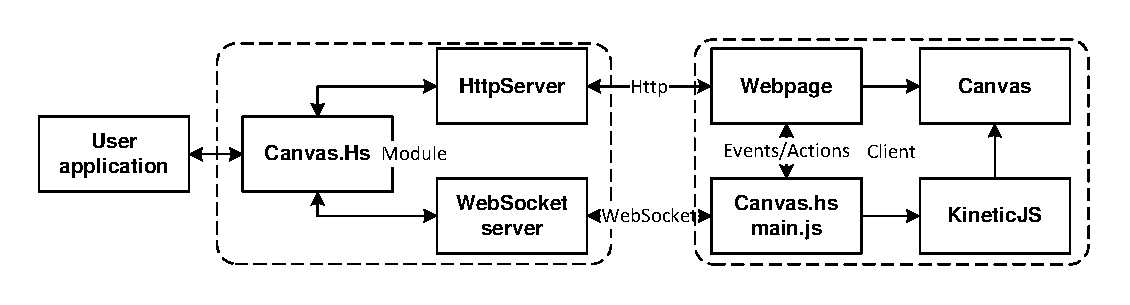
\includegraphics[keepaspectratio,width=\textwidth]{./images/architecture.pdf}
\caption{Architectuur van Canvas.hs}
\label{fig:architectuur}
\end{center}
\end{figure}

\subsubsection{Communicatie}
Gegevensoverdracht tussen de HTTP server en de browser moet snel gebeuren. Om de grafische elementen in de browser weer te geven moeten de output van de grafische interface naar de browser gecommuniceerd worden. Wanneer de gebruiker interactie heeft met de interface moet dit naar het programma van de gebruiker gecommuniceerd worden. Verder zal het programma bepaalde acties moeten kunnen uitvoeren op de webbrowser, zoals fullscreen laten gaan van de browser. Een belangrijke overwegingen is dat de grafische interface zo min mogelijk vertraging moet hebben.


\paragraph{Websockets}
Het is mogelijk om door middel van XMLHttpRequest of WebSockets een verbinding te onderhouden tussen de Module en de Clientomgeving. XMLHttpRequests worden door alle webbrowsers ondersteund, en kan door middel van longpolling technieken (Comet) \todo{PJ: wat is deze? of meer uitleg of verwijzingkje denk ik} een verbinding onderhouden met de webserver. De meest recente browsers ondersteunen WebSockets. Dit biedt een socket verbinding tussen de client en de server. Het WebSockets protocol biedt een betere performance dan alle technieken op basis van XMLHttpRequests en biedt een groter implementatiegemak. Door het gebruik van het HTML canvaselement zal de browser ondersteuning al beperkt zijn tot de meest recente browsers. Canvas.hs maakt gebruik van WebSockets.

\paragraph{Protocol}
In Cavas.hs wordt voor deze communicatie gebruik gemaakt van JSON \cite{JSON2006}. JSON staat voor JavaScript Object Notation en is een notatie waarin objecten als text worden gerepresenteerd zoals dit ook in Javascript wordt gedaan. JSON is een veel gebruikte notatie voor communicatie met Javascript. Het voordeel van JSON is, doordat het zo veel gebruikt wordt, dat er veel bibliotheken beschikbaar zijn om met JSON om te gaan. Zowel voor javascript als voor Haskell was het eenvoudig een goede externe bibliotheek te vinden om data van en naar JSON te lezen en te schrijven. Een ander groot voordeel van JSON is dat het, in tegenstelling tot bijvoorbeeld XML, weinig overhead heeft. Een uitgebreide handleiding van het protocol van gevonden worden in \cite{Protocol2013}.

Het protocol tussen de client en de server bevat voornamelijk interface data. De structuur en de attributen moeten vertaald worden van de Haskell omgeving om gebruikt te worden om te tekenen in het Canvas en vervolgens input van de gebruiker in de client te ondersteunen. De datastructuur van het protocol lijkt zoveel mogelijk op die van het canvas. Hierdoor kan data die binnenkomt bij de javascript applicatie zonder al te veel veranderingen op het canvas getekend worden.

\paragraph{Stateless module}
De Canvas.hs module houdt de huidige grafische boom niet bij. Deze wordt na ontvangst van de gebruiker applicatie onmiddelijk geëncodeerd naar JSON en opgestuurd naar de Javascriptapplicatie. Dit heeft een aantal voordelen, allereerst maakt dit het gebruik van de module door de programmeur gemakkelijker. Elke keer dat de eventHandler wordt uitgevoerd wordt hiervan verwacht dat deze een volledige grafische boom oplevert. Hierdoor is het voor de programmeur en de module niet nodig om uit te zoeken waar de grafische boom precies veranderd moet worden. Bijkomend voordeel hiervan is dat er slechts één plek is waar de huidige grafische boom wordt bijgehouden: de Javascript applicatie. Hierdoor kunnen er geen synchronisatiefouten tussen de Haskell module en de Javascriptapplicatie ontstaan. 

Nadeel van deze aanpak is dat er veel overhead is door het voortdurend versturen van de volledige grafische boom. Zelfs voor het verplaatsen van één object moet de hele boom opnieuw verstuurd worden. Dat er veel data verstuurd wordt levert geen problemen op doordat het systeem ontwikkeld is voor lokaal gebruik en data over websockets lokaal zeer snel verstuurd wordt. De aanpak levert wel problemen op als er snel veel getekend wordt, doordat het tekenen naar het canvas in onze aanpak relatief veel tijd kost. Hier wordt verder op gereflecteerd onder conclusie.\todo{Dit daadwerkelijk doen, referentie invoegen}
\subsection{Externe libraries}

\subsubsection{Webserver}
Om de statische files van onze library te serveren hebben we een HTTP-server nodig, we hebben hier gekozen voor ``warp''. Warp bied een lichtgewicht webserver die goed gedocumenteerd en ondersteund is. Andere opties waren ``happstack'', ``hyena'' en ``snap server"". Dit zijn eigenlijk volledige webframeworks, wij hoefden slechts statische files te serveren. Voor de eenvoud en onderhoudbaarheid was ``warp'' de beste keuze.

\subsubsection{Websocketserver}
De websocketserver is degene die connecties tussen de Haskell en Javascript onderhoud, we hebben hier gekozen voor de ``websockets'' library. Er had gekozen kunnen worden om hieromheen de ``wai'' wrapper te gebruiken, maar omdat we weinig gebruik maken van andere functionaliteit van ``wai'' hebben we het bij de normale library gehouden.

Binnen de websockets zijn er verschillende protocollen gedefineerd, welke in verschillende browsers geimplementeerd zijn. De meest recente versie van het websockets protocol poogt een standaard te worden (RFC6455) en de websockets library heeft daar tijdens ons ontwerpproject support voor gekregen. De meeste recente browsers hebben RFC-6455 geimplementeerd, en de verwachting is dat deze versie van het protocol lange tijd ondersteund wordt.

\subsubsection{JSON}
Binnen ons protocol gebruiken we JSON. In eerste instantie wilden we hiervoor een eigen parser schrijven, we waren namelijk sceptisch over het gebruik van een library omdat het parsen van JSON niet moeilijk lijkt terwijl de libraries ingewikkeld leken. Uiteindelijk hebben we toch een library genomen, libraries vertrouwde stukken code zijn waarvan al geverifieerd is dat ze werken, daartoe bespaart het ons veel tijd en hebben we een solide basis van onze code.

Er zijn voor haskell twee bekende JSON libraries, Text.JSON en Aeson. In eerste instantie hebben we gekeken naar Text.JSON maar al snel bleek dat deze library slecht gedocumenteerd is. Daarna hebben we naar Aeson gekeken, Aeson is beter gedocumenteerd en bied eenzelfde workflow.
Binnen Aeson is er gekozen om Template Haskell functies te gebruiken, dit is een GHC extensie die een soort van metaprogramming toevoegd aan Haskell. Template Haskell is gebruikt om lege keys uit de JSON te verwijderen en een record probleem van Haskell te omzeilen.

\subsubsection{Tests}
Als testingframework hebben we voor Hspec gekozen. Hspec intergreerd goed met andere testframeworks zoals QuickCheck en HUnit maar daarbovenop voegt het verhalende syntax toe aan de testcases. Ook zoekt Hspec automatisch naar testcases, en paralleliseerd het testcode.

Binnen Hspec maken we ook gebruik van QuickCheck, deze library kan arbitraire testcases testen. Hiervoor dient de input gedefineerd te worden en dan zal QuickCheck een groot aantal testcases loslaten op de code. Vaak gebruiken we eerst een voorgedefineerde testcase (van HSpec zelf, wat weer een wrapper om HUnit is), en daarnaast een arbitrair aantal extra testcases gegenereerd door QuickCheck. Zo weten we dat het geen toeval was dat onze tests checkte en kunnen we zonder al te veel moeite veel gevallen proberen.

\subsection{Module}
De module is de Haskell bibliotheek die de programmeur gebruikt om de grafische interface in de client te bedienen. Naar de programmeur is de gebruiksvriendelijkheid van de biblotheek een van de belangrijkste overwegingen voor het ontwerp. De module bestaat uit een aantal onderdelen: de server die de statische bestanden serveert, de websocket server die de verbinding met de client onderhoud, en de laag die de input en output verwerkt. \autoref{fig:architecture_module} geeft de architectuur weer van de module.

\begin{figure}
\begin{center}
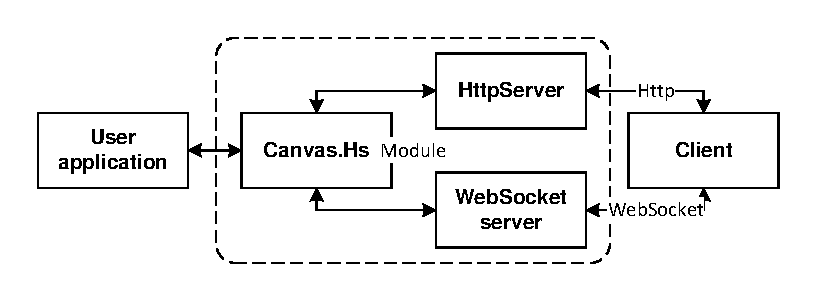
\includegraphics[keepaspectratio,width=\textwidth]{./images/module_architecture.pdf}
\caption{Architectuur van de module}
\label{fig:architecture_module}
\end{center}
\end{figure}

\paragraph{Servers}
Canvas.hs draait een simpele server op port 80 die statische bestanden kan serveren. Waaronder de index pagina, de javascript bestanden en eventueel plaatjes. Op port 8080 draait een websocket server die de verbinding met de client onderhoud.


\paragraph{Server in de module}
De server draait in het process wat gestart wordt vanuit de Haskell-code van de programmeur. De main van de programmeur start (indirect) de server. Dit is envoudiger dan het draaien van de server in een apart process. Er hoeft namelijk niet tussen verschillende Haskell-processen gecommuniceerd te worden. Dit scheelt het schrijven van nog een interface tussen het server- en het module process. Nadeel is wel dat het voortdurend opnieuw starten en afsluiten van de server leidt tot vertraging in het opstarten van het programma van de programmeur. Dit is vervelend als de programmeur regelmatig kleine wijzigingen maakt en dan de code opnieuw moet starten. Echter lijkt de overhead van het opnieuw starten van de server minimaal. Het is verder praktisch dat er geen rekening gehouden hoeft te worden met de state van de server bij het opstarten van het programma.

\paragraph{Gebruik} Wanneer de programmeur gebruik wil maken van de Canvas.hs moet hij gebruik maken van de installEventHandler functie. Bij het aanroepen van deze functie moet de programmeur een event handler meegeven die alle events vanuit de interface afhandeld. Om het gebruik van Canvas.hs zo makkelijk mogelijk te houden zal bij het aanroepen van installEventHandler automatisch de statische server en de websocket server gestart worden, en daarna automatisch de browserpagina geopend worden. \autoref{fig:startup_procedure} geeft de opstartprocedure weer.

\begin{figure}
\begin{center}
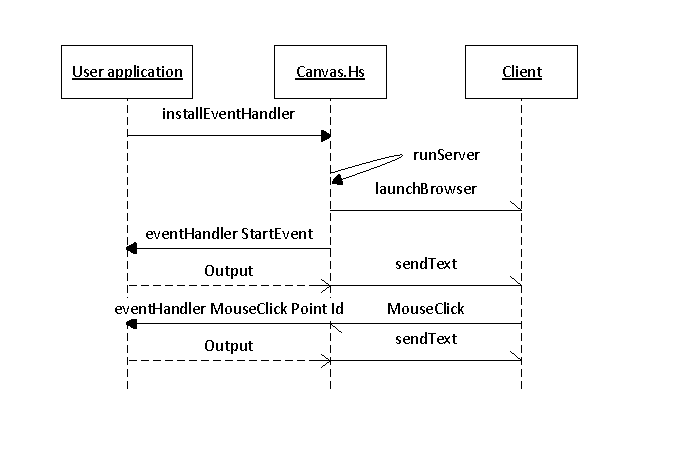
\includegraphics[keepaspectratio,width=\textwidth]{./images/module_startup_procedure_interaction.pdf}
\caption{De opstartprocedure en initiele interactiesequentie}
\label{fig:startup_procedure}
\end{center}
\end{figure}

\paragraph{Input/output}
De module handeld input en output af door events naar de eventhandler van de programmeur te sturen. Bijvoorbeeld: wanneer een gebruiker op een rondje klikt zal het programma de event handler aanroepen met de ID van dat rondje en de lokatie van de muisklik. De event handler van de programmeur kan dan nieuwe output genereren op basis van dit event. Zoals een nieuw menu weergeven of het uitvoeren van een actie zoals het opvragen van een bestand van de gebruiker.In \autoref{fig:startup_procedure} is deze interactie weergegeven.

De programmeur zal in zijn eventhandler bij ieder event de huidige state en de huidige event meekrijgen. Het type van de eventhandler is \inlinecode{userState -> Event -> (userState, Output)}, waarin de programmeur elk type aan userState kan geven. Door middel van pattern matching kan de programmeur makkelijk een bepaald event opvangen. Een muisklik event wordt opgevangen door: \inlinecode{handler state (MouseClick (x,y) "id")}. De returnwaarde vand de eventhandler is een tuple van de nieuwe state en de output. Output is een tuple van \inlinecode{(Maybe Shape, [Action])}. De eventhandler kan meerdere acties tegelijk uitvoeren en/of een grafische output leveren. De ondersteunde events en outputtypes worden verder toegelicht in \autoref{subsec:grafische_bibliotheek}.

-TODO: Acties   
\paragraph{Timers}
Canvas.Hs ondersteund timers die ervoor zorgen dat met een bepaald interval een event naar de eventhandler wordt verstuurd. Hiermee kunnen bijvoorbeeld animaties worden toegevoegd aan de interface. Deze timers worden bijgehouden in de module. Een alternatief is om de timers aan de client over te laten. Dit heeft als voordeel dat het makkelijker is om timers bij de houden in JavaScript dan in Haskell. In Haskell ontstaan er dan verschillende threads die je moet bijhouden. Groot voordeel is dat er geen extra acties over de WebSocketconnectie verzonden hoeven worden en dat een implementatie direct in Haskell meer precisie geeft voor de timer.

\paragraph{Unsafe I/O}
In Server.hs wordt gebruik gemaakt van unsafePreformIO voor het starten van child processen (een MVar die threads bijhoudt) en om een verbinding met een client bij te houden (een IORef die de connections naar de clients bevat). Hoewel het in dit geval volkomen veilig is, zijn er bezwaren tegen het gebruik van unsafePerformIO\cite{Haskell.org2008}. Dit is namelijk niet de netste oplossing en kan meestal voorkomen worden. Het is netter om een Server Monad te gebruiken die een State implementeert die deze zaken bijhoudt. Echter is het implementeren daarvan tijdsintensief, waardoor voor deze oplossing is gekozen.

\subsection{Client}
Het voornaamste onderdeel van de client is het canvas-element waarin de output getekend wordt door Kinetic.js. Daarboven zit de Canvas.hs javascriptcode die de verbinding onderhoud met de module en dit doorspeeld naar Kinetic.js om te tekenen. In dit deel worden voornamelijk de ontwerpbeslissingen besproken die betrekking hebben op de werking met KineticJS en de webbrowser.

\begin{figure}
\begin{center}
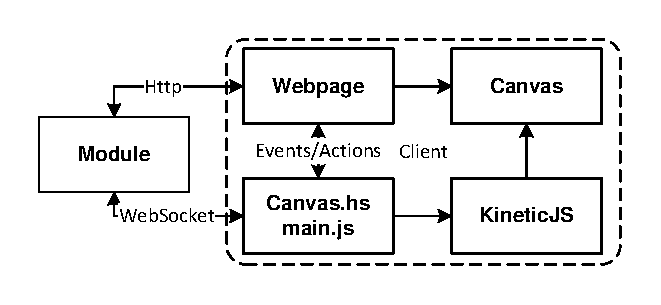
\includegraphics[keepaspectratio,width=\textwidth]{./images/client_architecture.pdf}
\caption{Architectuur van de JavaScript client}
\label{fig:architecture_client}
\end{center}
\end{figure}

\subsubsection{Canvas/Events}
Vanuit de module ontvangt de client via de WebSocket verbinding output. Ieder element wordt omgezet en aangemaakt in KineticJS. Voor elk element dat geinteresseerd is in een event wordt een eventlisteners toegevoegd. Wanneer de volledige structuur opgebouwd is wordt door oude structuur weggegooid en de nieuwe structuur op het canvas getekend.

\paragraph{Mousedrag}
Standaard ondersteund KineticJS mousedrag events, maar door de manier waarop Canvas.hs iedere keer opnieuw de output genereert raken de events van KineticJS verloren. Daarom maakt Canvas.hs gebruik van een eigen implementatie van mousedrag in de Canvas. Een mousedrag begint met een MouseDownEvent. Vanaf dat moment houd de client een ID bij van het huidige element. Alle opvolgende MouseMoveEvents zijn drag events die naar de client worden verstuurd. Deze MouseMoveEvents worden dooregegeven naar de Haskell kant met de vorige coördinaten van de muis en de huidige coördinaten van de muis.
Op deze manier kan de Haskell kant bepalen wat er moet gebeuren tijdens het draggen. Op het moment dat het programma aangeeft niet meer geinteresseerd te zijn in drag events op dat ID of in het geval van een MouseUpEvent stopt de drag in de client.

\subsubsection{Acties}
De programmeur kan een aantal specifieke acties uitvoeren op de client. De state van deze acties wordt onderhouden door de client zelf.
-TODO: Referentie naar de specifieke sectie in de grafische bibliotheek

\paragraph{Browserrestricties}
Canvas.hs bied de optie om de canvas in volledigscherm te laten weergeven. Door veiligheidsfunctionaliteiten in de huidige webbrowsers is het niet mogelijk om direct naar volledigscherm te gaan met behulp van JavaScript. Dit is alleen mogelijk vanuit klik- en toetsenbordevents. Daarom krijgt de gebruiker eerst een menu te zien voordat de browser naar volledigscherm gaat. Dezelfde veiligheidsrestricties zijn er voor het bestandenselectiemenu hierdoor heeft Canvas.hs daar ook een menu voor.

-TODO: Referentie naar de grafische bibliotheek over volledigscherm

\paragraph{Debug Console}
Voor de programmeur die gebruik gaat maken van de Canvas.hs library is het belangrijk dat zijn interface er zo uit ziet zoals hij dit wil. Ongetwijfeld zal een programmeur tegen problemen aanlopen bij het bouwen van de interface die hij niet had voorzien bij het schrijven van zijn code. Om probleemoplossing hiervan te vergemakkelijken bevat Canvas.hs een debug console bevat waar het aanroepen van teken functies en de invloed van deze API aanroepen goed visueel en tekstueel inzichtelijk worden. Doormiddel van een actie vanuit het programma van de gebruiker kan de debug console tevoorschijn gehaald worden.
\subsection{Problemen}

Bij het ontwerp en implementatie van het project zijn er een aantal moeilijkheden geweest die het uiteindelijke ontwerp van Canvas.hs sterk hebben beïnvloed. Deze ontstonden onder andere door het ontwijken van het gebruik van monadisch programmeren voor de student en door de samenwerking tussen Haskell en Javascript. Hieronder een kort overzicht van deze belangrijkste problemen.

\subsubsection{Haskell interface}
Doordat zowel het tekenen van grafische elementen als het uitvoeren van IO acties normaal gesproken via (een monadlaag op) de IO-monad verlopen moet Canvas.hs deze beide mogelijk maken. Hierdoor is de interface voor de user applicatie erg uitgebreid. 

Er moest een manier gevonden worden zodat de handler zowel acties als grafische elementen kon opleveren, en het ook mogelijk is om slechts één van beide door te geven. Dit is gedaan door deze te verpakken in een tuple van een te tekenen grafisch element en een lijst van uit te voeren acties. Helaas resulteert dit in de user application in code die niet altijd even goed leesbaar is, daarom zijn er een tweetal hulpfuncties in het leven geroepen, \inlinecode{shape} en \inlinecode{actions}, die de leesbaarheid in de user application verhogen.

\paragraph{Acties met resultaat}
Naast het bovenstaande is er nog een probleem met acties. Sommige acties hebben geen resultaat, zoals bijvoorbeeld het aanzetten van de Debug-console, of ze hebben pas later resultaat, zoals bijvoorbeeld het starten van een Timer of het vragen om een bestand van de gebruiker. Echter zijn er ook acties, zoals het openen van een bestand, die onmiddellijk resultaat opleveren. 

Dit laatste type actie kan niet met een grafische boom gecombineerd worden. Als dit wel toegestaan zou zijn kan er een onduidelijkheid ontstaan. De actie zou dan worden uitgevoerd en een resultaat opleveren dat vervolgens weer door de user applicatie wordt verwerkt. Hieruit zou weer een nieuwe grafische boom kunnen komen. Er zijn dan twee aparte grafische bomen, waarvan er slechts één naar de Javascript applicatie kan worden gestuurd. De user applicatie zou zelfs weer zo'n actie op kunnen leveren, waardoor er drie te versturen grafische bomen zouden kunnen liggen, etc. 

Er is daarom voor gekozen om de acties in twee types op te delen, acties die geen direct resultaat (\inlinecode{Action}) op leveren en acties die direct resultaat op leveren (\inlinecode{BlockingAction}). Van dit eerste kunnen er zoveel worden opgegeven als gewenst en deze kunnen gecombineerd worden met een te tekenen grafisch element. Het tweede type kan niet met een grafische boom gecombineerd worden en het resultaat kan ook uit slechts één zo'n actie bestaan. 

\subsubsection{Aannamen gebruik}
Bij het ontwerp van Canvas.hs is uitgegaan van de ervaring van de ontwerpers bij het vak functioneel programmeren. Veel ontwerpkeuzes zijn gemaakt rond het principe dat de interface van Canvas.hs zo simpel mogelijk moet zijn voor de student. Zo is er zo veel mogelijk gekozen voor simpele primitieven als String en Int. In het geval van interactie met de inhoud van bestanden, is gekozen voor het gebruik van Lazy ByteStrings om interactie met de inhoud mogelijk te maken zonder het hele bestand in het geheugen te laden.

Er is voor gekozen om geen gebruik te maken van het Num-type uit fpprac. Zo is Canvas.hs ook bruikbaar zonder gebruik te maken van fpprac. Het is echter eenvoudig om in fpprac een koppeling met Canvas.hs te schrijven die gebruik maakt van het Num-type.

\subsubsection{Verschillen systemen}
Doordat er bij het tekenen van de grafische elementen gebruik wordt gemaakt van javascript en canvas in de browser van de gebruiker ontstaan er door inconsequenties tussen bugs in browsers en besturingssystemen een aantal problemen. Veel van deze problemen hebben we opgevangen door gebruik te maken van bibliotheken aan de Javascript kant als jQuery en KineticJS. 

\paragraph{Systeemtoetsen} Echter zijn er een aantal zaken waar systemen zo in verschillen dat we deze niet voor alle mogelijke systemen hebben afgevangen in Canvas.hs. Er zijn bijvoorbeeld grote verschillen in de toetsenborden tussen verschillende systemen. Zo heeft windows een windows-toets, OS X een command-toets en noemen de meeste Linux distributies deze knop de super-toets, we hebben er in Canvas.hs voor gekozen al deze toetsen onder de naam 'superkey' te scharen.

\subsection{Grafische bibliotheek} \label{subsec:grafische_bibliotheek}

-TODO: Ontwerpkeuze: Referentie van specifieke elementen met behulp van ID toelichten
